\documentclass[12pt,a4paper,twoside,openright,bibliography=totocnumbered]{report}

\usepackage{ragged2e}
\usepackage{tikz, pgfplots}
\usepackage{graphicx}
\usepackage{multicol}
\usetikzlibrary{positioning,shapes}
\usepackage{graphicx}
\usepackage{url}
\graphicspath{{./reportImages/}}
\usepackage{geometry}
\usepackage{listings}
\usepackage{amsmath}
\usepackage{tcolorbox}
\usepackage{enumitem}
\usetikzlibrary{arrows.meta, positioning}
\usepackage{amssymb}
\usepackage{setspace}
\usepackage{titlesec}
\usepackage{times}
\usepackage{tocbibind}
\usepackage{subcaption}
\usepackage{tabularx}
\usepackage{array}
\usepackage{booktabs} % For better table formatting
\usepackage{float}
\usepackage{algorithm}
\usepackage{algorithmic}
\usepackage{varwidth}
\usepackage{pgfplots}
\usepackage[export]{adjustbox}
\pgfplotsset{compat=1.18} % Adjust version compatibility as needed
%\usepackage[usenames,dvipsnames]{xcolor} % to access some named colors used with \highLight
%\usepackage{luacolor} % required to use the lua-ul \highLight command
%\usepackage{lua-ul}

%\LuaULSetHighLightColor{Aquamarine}

\setlist[itemize]{noitemsep, topsep=5pt}

\newcommand{\notimplies}{\;\not\!\!\!\implies}

\geometry{margin=1in}

\lstdefinestyle{st1}{
	numbers=left,
	tabsize=2
}

\lstset{style=st1}

\title{Optimizing Computational Graphs Using Relaxed Graph Substitutions}

\author{Kaushik Bhowmick\\ \texttt{u21cs022@coed.svnit.ac.in}
		\and
		Himanshu Thakur\\ \texttt{u21cs046@coed.svnit.ac.in}
		\and
		Bhavya Hirani\\ \texttt{u21cs100@coed.svnit.ac.in}
		}

\date{\today}

\onehalfspacing


\begin{document}
%\maketitle

%\begin{center}
%{ \Large \bfseries Building a test case for Interprocedural GVN } \\
%\end{center}
\pagenumbering{Roman}

\begin{singlespace}
\begin{footnotesize}
\begin{abstract}
\thispagestyle{plain}
\setcounter{page}{3}
	\textit{Most deep learning compilers use a greedy approach to optimizing computational graphs in that every successive graph substitution must result in a strict performance increase. This narrows the space of possible optimizations and motivates the notion of relaxed graph substitutions: substitutions that don't themselves necessarily result in a more optimal computation graph, but facilitate further transformations down the line that ultimately yield a net improvement in performance. In order to determine the sequence of transformations to be applied such that the net performance increase is guaranteed, we search the space of potential optimizations using a backtracking algorithm which, at a given iteration, determines the cost of the corresponding intermediate graph using programmer-defined heuristics in the form of a cost-model. To test our optimization strategy, we plan to implement our own graph transforms in Open Neural Network Exchange (ONNX) and we limit our performance heuristics to simply measuring inference time. So far we have created arbitrary computation graphs in ONNX and furthermore successfully implemented the 'enlarge kernel size', and 'fuse conv layers' transforms on it. We have implemented a Floating Point Operations Per Second (FLOPS)-based cost-model to benchmark our model without the need to actually run it. It is fairly accurate in estimating real inference times as we detail in our results. All this is integrated into a cost-limited backtracking algorithm which programmatically discovers new relaxed graph substitutions. Further we have unpacked the theoretical the details of two more transforms - fusing two convolutional layers and fusing an add and convolutional layer.}\\
\end{abstract}
\end{footnotesize}
\end{singlespace}

\tableofcontents

\listoffigures

\titleformat{\chapter}[display]
        {\normalfont\Large\bfseries\centering}
        {\chaptertitlename\ \thechapter}
        {20pt}{\Large}

\titleformat{\section}[hang]
        {\normalfont\normalsize\bfseries}{\thesection}{0.5em}{}

\titleformat{\subsection}[hang]
        {\normalfont\small\bfseries}{\thesubsection}{0.5em}{}

\chapter{Introduction}
\pagenumbering{arabic}
\setcounter{page}{1}
%{\large \noindent \bfseries  Introduction}\\
In most Deep Learning (DL) frameworks, training and inference are both represented using \textit{Computation Graphs}, where nodes represent operations, and edges represent the flow of data through those operations. Particularly, we can think of each incoming edge for some node N representing arguments to N, each argument being the result of computing the respective subgraphs they are the roots of. Computation graphs, like other programs, can usually be optimized for some metric such as optimal memory usage or efficiency, and has motivated a vast body of literature surrounding the same. That being said, most, if not all, optimizations being worked on so far have been \textit{greedy} in nature. i.e. They optimize a program in \textit{passes}, where each pass, i, goes over the program in order to make some transformation $T_i$, such that $T_i$ \textit{must} lead to a strict performance increase. 

The described constraint restricts the space of transformations an algorithm must explore, and, presumably, sacrifices a hard-to-discern, but ``globally optimal'' solution for a possibly locally optimal option that is guaranteed to improve performance within some time constraint. The idea behind \cite{jia2019} is that it's very feasible to search in a much bigger search space of what are called \textit{relaxed graph substitutions}, leading to a discovery of complex substitutions that go through potentially sub-optimal intermediate steps (hence, ``greedy'') to reach an ultimate resultant computation graph that is better than what we would have achieved using greedy strategies.

The approach presented here is a backtracking algorithm that searches the exhaustive space of intermediate graphs obtained by applying all possible transformations on them (regardless of reducing performance, assuming the reduction in performance is below a set tolerance criteria). To quantify the performance of these intermediate graphs, so as to compare it with its predecessor, successor and other interemdiate transformations, we also need a \textit{cost model} that allows us to statically estimate the same.

\section{Objectives}
Our objectives with this project are two fold:
\begin{enumerate}
	\item Replicate results obtained by \cite{jia2019}, but without the graph splitting algorithm (used to scale the aforementioned non-greedy approach for large graphs)
	\item Flesh out the \textit{cost model} which statically estimates performance metrics on intermediate graphs.
\end{enumerate}
	
\noindent The report is organized as follows:
Chapter 2 gives some theoretical background on deep learning compilers and our motivation for exploring this particular thread of research. Chapter 3 gives some detail about our algorithm, including an in-depth explanation on a running example that we plan to impement as a demonstration of the algorithm. Chapter 4 provides some insight into possible challenges one can face when implementing such a scheme, along with future directions we plan to follow. Chapter 5 summarizes and concludes our exposition.


%We use an example from a ResNet \cite{he2016} module ( figure \ref{resnet} ) to illustrate our strategy. Each arrow represents a graph substitution that produces a graph \textit{equivalent} to its input, where equivalence is defined as the following: two graphs $\mathcal{G}_1$ and $\mathcal{G}_2$ are said to be equivalent if they produce the same outputs for an arbitary input. The first substitution pads a 1x1 convolutional kernel to form a 3x3 one, potentially reducing the performance by introducing more operations. However, doing so enables further node fusions which, as we can see, results in a computational graph giving better performance than what we started with. \\


%\begin{figure}[b!]
	%\begin{center}
		%\includegraphics[scale=0.3]{resnetExample}
	%\end{center}	
	%\caption{An example from \cite{jia2019} that demonstrates a relaxed graph substitution}
	%\label{resnet}
%\end{figure}

%%\pagebreak

\chapter{Theoretical Background and Literature Review}
%{\large \noindent \bfseries  The Backtracking Algorithm}\\

\section{Deep Learning Compilers and Motivation}
In this section, we give an overview of the general landscape of deep learning compilers, and motivate the need for the endeavor we choose to embark on. Deep Learning compilers essentially aim to specialize existing, but hitherto general, compilation techniques, so as to perform optimizations specific to deep learning and machine learning workloads. Here by \textit{general}, we mean techniques that can be applied across the board for any language as long as it's first converted to some suitable intermediate representation (assuming the transforms need such a requirement, such as the Intermediate Representation (IR) being LLVM IR\cite{lattner2004llvm}). Since deep learning computational graphs are usually very uniform and limited in terms of their basic operations, optimizing specifically for them becomes not only reasonably tractable but also beneficent. 

\subsection{Intermediate Representations and The current Optimization Scenario}
According to \cite{li2020deep}, a rather generalized pipeline for compilation frameworks, which are much more amenable to such specializations as deep learning, is emerging in the form of MLIR \cite{lattner2021mlir}. The notion behind such a pipeline can be described in the following way:
\begin{itemize}
	\item Computation graphs are usually defined at a coarse granularity consisting of abstract operations such as convolutions and pooling. While improvements can be made by altering graphs on this level, the abstraction makes doing so quite restricting.
	\item On the other hand, when compiled to intermediate representations such as LLVM IR, the operations not only lose their abstraction, but they plummet to a level no longer reminiscent of the domain they are actually specific too, and so nothing can be done beyond general optimizations whicha are anyways done on general purpose languages like C++ or Java. The idea is that different sized ``chunks'' of this IR represent algorithms or structures that are (i) used exclusively in our domain, such as a convolution algorithm (ii) are at an abstraction level lower than or equal to that of computation graphs. If we could somehow expose these ``chunks'' so that they were explicit operations at a level of abstraction below computation graphs, but above machine code, opportunities exist for much more optimization!
	\item MLIR does exactly this, by allowing users to specify multiple, custom, intermediate representations, called \textit{dialects}, which can be deployed seemlessly into a pipeline where one can iteratively lower from one IR to another, doing any necessary processing on the way.
	\item Having these different IRs, exposes potential for optimizations at different levels.
\end{itemize}

Many deep learning compilers \cite{hloir} \cite{halideir} exploits one of these ``levels'' of interemediate representations to do domain specific optimizations. If done at a lower level, they could be optimized for, say, deep learning hardware like Google's Tensor Processing Units (TPUs) \cite{jouppi2017datacenter}, and if done at a higher level, they may represent, say, operations such as fusing two convolutions.


\subsection{Motivation for Non-Greedy Approaches}
Research in deep learning compilers is vast and rapidly growing. The following are some directions in which recent work has been done:
\begin{itemize}
	\item \textbf{Optimizing for domain-specific hardware, like TPUs.} This includes the creation of IRs specific to an application or hardware. For example, the work by Hu et al.\cite{hu2023tpumlircompilertpuusing} defines two new MLIR dialects, TOP and TPU, that successively perform different kind of optimizing passes specific to a TPU. Given their passes are atomic and by definition "optimizing", their approach is also a greedy one. Furthermore, OpenVINO \cite{openvino} by Intel optimizes models specifically for Intel hardware. 
	\item \textbf{Evolving algorithms that specialize on particular kinds of inputs.} For example, Graph Neural Networks \cite{wu2024hector}, which are build specifically to make explicit, graph-like relations in a given problem. These techniques have optimizations inherent in the actual Deep Neural Network (DNN) rather than doing them as some sort of post processing, which means greedy or non-greedy algorithms don't come into the picture.
    \item \textbf{Optimizing Distributed DNN training.} Recent advancements have introduced deep learning frameworks designed to automatically identify efficient parallelization strategies for distributed DNN training. For instance, ColocRL \cite{mirhoseini2017device} employs reinforcement learning to determine optimal device assignments for model parallelism across multiple GPUs. Similarly, FlexFlow \cite{jia2019beyond} explores an extensive range of parallelization strategies and utilizes randomized search to identify effective solutions within this space. However, these works all assume a fixed computation graph, and find ways of distributing said graph better, which doesn't consider a reduction in the inherent computational cost of deep neural networks, and hence doesn't fit into the direction we wish to explore.
    \item \textbf{Verification and Repair of Deep Neural Networks}. By its nature, verification involves giving theoretical guarantees on certain optimizations, which means the prospect of "allowing degradation" doesn't come into the picture, unless it is a part of the proof that proves the improvement. An example is \cite{vthakurverified}.
\end{itemize}

With this literature survey, however, we found that the assumption relating to greedy transformations held true for many cases, and little information was available on non-greedy approaches to optimizing programs. Furthermore, most, if not all, of the aforementioned threads of research already have working implementations on well-reputed libraries such as TensorFlow \cite{tf2016}, PyTorch \cite{pytorchdocs}, and ONNX Runtime \cite{onnxoptimizer} and hence, wouldn't benefit much from another nudge in that same direction. With that in mind, we aim to explore this space of greedy optimizations and replicate results given in \cite{jia2019}.

\subsection{Estimating Computational Graph Costs}
One of the primary components of our work is a program that takes a DL computational graph as input, and gives us, as output, an estimation of its execution time, without actually running the graph. This component is called the \textit{cost model}. While the cost model is essential to this project (as we'll soon see), estimating computational graph costs is a problem that has been explored many times before (as we shall see in a moment) for the following reason:
When neural network architectures have a large inference time, testing various architectures for any given application, so as to select the optimal architecture, becomes a slow and tedious task. Being able to estimate graph costs without running the actual inference, hence, is a valuable tool to have at one's disposal.
We can categorize the approaches taken for estimating neural network inference times into two broad categories: (i) Hardware agnostic and (ii) Hardware sensitive

\begin{enumerate}
    \item The tools that are hardware agnostic estimate graph costs without considering hardware-level intricacies that play a role in the performance of certain algorithms. For instance, the Very Large Instruction Word (VLIW) length or specific Instruction Set Architecture (ISA) instructions might make an algorithm run faster on one architecture compared to the other. If we were to consider these, the developer using this tool would have to specify the required hardware parameters such as bandwidth, cores, etc. before using the tool to estimate costs. Our approach in this paper has been majorly derived from the work done in \cite{qi2017paleo} and \cite{osterwind2022hardware}. We consider aspects that may affect performance at a granularity coarser than architectural details. This has an advantage in that the tool may be used for all platforms with minimal overhead. 
    \item The lines between hardware agnostic and sensitive are a little blurred. ANNETTE \cite{wess2020annette} uses an approach, that, while hardware agnostic at its core, needs us to specify a lot of metadata about the device being used. It then takes about 3-5 days for the tool to benchmark appropriate hardware parameters which aid graph cost estimation. PerfNet \cite{wang2020perfnet} uses a Neural Network to estimate graph costs, and requires one to feed many details about the device to run inference. The advantage of using a more hardware sensitive approach is, of course, that the finer granularity lends us greater precision in most cases. 
\end{enumerate}

That being said, the above approaches rightfully try to get their cost estimates as close to the benchmarked cost as possible. This is not a constraint for our application, because, as we shall see later in this report, we only care about the relative graph costs between a set of candidate graphs. This encouraged us to use a hardware agnostic, rather than hardware sensitive approach in our work.


%{\large \noindent \bfseries  Proposed Methodology}\\
\chapter{Proposed Work}

There are essentially three major facets involved in coming up with an implementation for relaxed graph substitutions: (i) introducing "downgrading" graph substitutions that are likely to reduce the graph's performance, (ii) a backtracking search algorithm that searches the set of all possible semantically correct graph transformation sequences, and (iii) the cost function we will use to guide our backtracking search. We now describe the motivation for each of these steps in detail.

\section{Motivating our Approach Using an Example}
We use an example from a ResNet \cite{he2016} module ( Figure \ref{resnet} ) to illustrate our strategy. Consider feeding the the first graph in Figure \ref{resnet_a} to a state-of-the-art deep learning compiler such as TensorFlow RT. Such a compiler will detect that the two initial convolutions (say \textit{Conv1} and \textit{Conv2}) have the same attributes (kernel size, channels, input shape etc.), and can be \textit{fused} into a single convolution combining the channels from both those convolutions. 

However, what if the kernel sizes of \textit{Conv1} and \textit{Conv2} didn't match? In Figure \ref{resnet_b}, the convolutions in the leftmost graph won't be fused because their kernel sizes aren't compatible (\textit{Conv2} now has a 1x1 kernel instead of the earlier 3x3). That being said, there does exist a two-step method to optimize this graph: As the first step, we can pad the 1x1 kernel to form an \textit{equivalent} 3x3 kernel --- a step that causes a performance degradation due to increased computations. Doing so now allows us to fuse these kernels and save us the memory latency being spent on reading/writing tensor inputs/outputs. It so turns out, that the benefit obtained in Step 2 outweighs the loss incurred by step 1, resulting in a graph more optimal than our starting point.

\begin{figure}[ht!]
	\begin{subfigure}{\textwidth}
        \centering
		      \fbox{\includegraphics[scale=0.3]{resnetSubset_a}}	
        \caption{Most Deep Learning compilers will detect pairs of convolutions having the same attributes, and fuse them into a single convolution as an optimization step.}
        \label{resnet_a}
    \end{subfigure}
    \begin{subfigure}{\textwidth}
        \centering
            \fbox{\includegraphics[scale=0.3]{resnetSubset_b}}
        \caption{An example from \cite{jia2019} that demonstrates a relaxed graph substitution. If given the left graph, most compilers cannot perform the shown 2-step process to reach the optimized (right) graph, because the first step requires a "downgrading" graph transform.}
        \label{resnet_b}
    \end{subfigure}
    \caption{Difference between regular and relaxed graph substitutions.}
	\label{resnet}
\end{figure}

Optimization algorithms in modern compilers won't do the aforementioned two-step process because they do not have the "foresight" to look beyond a single transformation step: If optimality in the next step is not a theoretical guarantee, that transform is not done even if though it may lead to a better globally optimal solution as discussed (the latter may or may not be a theoretical guarantee). In other words, these algorithms search for optimizing \textit{transformations}, and not \textit{sequences of transformations}. By definition, this is a \textit{greedy} approach to optimization, and severely restricts the space of opportunities as shown. 

The above examples show two out of four total steps in this particular optimizing sequence. In the interest of brevity, we defer an explanation of the sequence to Appendix A.

\section{Defining our Goals}
In this study, we're particularly interested in the kind of optimizations facilitated by an initial reduction in performance, because removing this property leaves us with cases most compilers will optimize anyways. Therefore, our \textbf{first goal} is to introduce "deprecating" transformations in our list of optimizations. Once we have such a list of transformations, we can define our \textbf{second goal} as coming up with an algorithm that iterates through the space of transformation sequences with an aim of finding one that leads to a more optimal graph. That being said, knowing whether or not a given sequence is optimizing will require a comparison between initial and final computational graphs. Inference time cannot be used for such a comparison because the number of sequences to test will be very large. There needs to be a fast way to compare the efficiency of two computational graphs without running them. This brings us to our \textbf{third and most important goal} of defining a \textit{cost model} that approximates the cost of a given computational graph. These goals are summarized in Table \ref{tab1}.

\renewcommand{\arraystretch}{1.5} % Adjust vertical padding (1.5x default)
\setlength{\tabcolsep}{10pt} % Adjust horizontal padding

\begin{table}[]
    \centering
    \begin{tabularx}{\textwidth}{|>{\centering\arraybackslash}X|>{\centering\arraybackslash}X|}
        \hline
        \textbf{Description} & \textbf{Solution} \\
        \hline
        Introduce “downgrading” graph transformations that may lead to a better optimizing sequence compared to the “regular” strategy. (These are the only kind of cases we’re interested in investigating) 
        & TensorFlow transformations + Custom ones \\
        \hline
        Explore the space of possible sequences with the complete (optimizing+downgrading) set of transforms 
        & Backtracking Algorithm \\
        \hline
        Find a way to estimate one sequence is better than the other. (We can never know for sure without running) 
        & Cost Model (our primary goal) \\
        \hline
    \end{tabularx}
    \caption{Goals of This Study}
    \label{tab1}
\end{table}

\section{The backtracking Algorithm} \label{backtracking}
We take the following approach to search through the space of possible graph transformations:
		\begin{enumerate}
			\item Consider a list of possible graph transformations, $T$. At any given point in the algorithm, let $\mathcal{G}$ be the current intermediate graph version. We maintain a priority queue of intermediate graphs, ordered by their \textit{cost}, defined by a heuristic (in our case, this is simply the execution time).
			\item In each iteration:
				\begin{enumerate}
					\item We dequeue to get the next candidate intermediate representation $\mathcal{G}$. 
					\item For each optimization $t_i$ in $T$, we apply $t_i$ on $\mathcal{G}$ to obtain some equivalent graph $\mathcal{G}'$. If $cost(\mathcal{G}') < cost(\mathcal{G})$, we set $\mathcal{G} = \mathcal{G}'$. Else if $cost(\mathcal{G}') < \alpha \cdot cost(\mathcal{G})$, where $\alpha$ is a hyperparameter defined by the user (greater than one), then $\mathcal{G}'$ is considered to be a valid candidate for further search, and is added to the priority queue.
					\item $\alpha$ helps define how much of a performance decrease we can tolerate. This value can't be too high so as to avoid blowing up the search space, and hence, the time it takes for our algorithm to find a beneficial sequence of graph transformations.
				\end{enumerate}

			\item The above is repeated until there are still graphs to process in the queue.
		\end{enumerate}

Here, in 2(b), the factor $\alpha$ can be thought of as the amount of performance degradation we can tolerate for any given transform. This limit is important to cut down the space of possible sequences to a pragmatic value. The complete process can be seen in Algorithm \ref{alg:backtracking}

\begin{algorithm}[H]
\caption{Backtracking Search Algorithm}
\label{alg:backtracking}
\begin{algorithmic}[1]
\REQUIRE An initial model $G_0$, a cost function $\text{Cost}(\cdot)$, a set of valid operations $\{S_1, \dots, S_m\}$, and a hyperparameter $\alpha$.
\ENSURE An optimized model $G_{\text{opt}}$.
\STATE Initialize a priority queue $Q$, where models are sorted by $\text{Cost}(\cdot)$.
\STATE $Q \gets \{G_0\}$
\STATE $G_{\text{opt}} \gets G_0$
\STATE $C_{\text{opt}} \gets \text{Cost}(G_0)$
\WHILE{$Q \neq \emptyset$}
    \STATE $G \gets Q.\text{dequeue}()$
    \FOR{each operation $S_i \in \{S_1, \dots, S_m\}$}
        \STATE Apply $S_i$ to $G$ to generate a new model $G'$
        \IF{$\text{Cost}(G') < \text{Cost}(G_{\text{opt}})$}
            \STATE $G_{\text{opt}} \gets G'$
            \STATE $C_{\text{opt}} \gets \text{Cost}(G')$
        \ENDIF
        \IF{$\text{Cost}(G') < \alpha \cdot C_{\text{opt}}$}
            \STATE $Q.\text{enqueue}(G')$
        \ENDIF
    \ENDFOR
\ENDWHILE
\RETURN $G_{\text{opt}}$
\end{algorithmic}
\end{algorithm}

\section{The Cost Model}
		
		% Explain the need for evaluating it statically
		% FLOPS
		% Execution time
		
	When comparing the expected performance of intermediate graphs, $\mathcal{G'}$, we cannot simply run the inference on them and compare execution times because an exhaustive search will go through a vast number of potential graphs. Running them will not only result in an enormous amount of computation overhead, but also might involve convoluted problems related to memory latencies and slow I/O operations, making such a strategy quite impracticable. Furthermore, it might be better to have an algorithm that is more amenable to a flexible cost function, that optimizes for not necessarily execution time, but also other metrics such as Floating Point Operations (FLOPS) or Memory accesses. As a result, a flexible, static cost estimation strategy must be developed. 
	
    Estimating the cost would ideally have to be done by taking many hardware factors into consideration, since the Instruction Set Architecture (ISA) and the nature of the processors would greatly affect what kind of computations can be done faster, say. However, fine-tuning algorithms to specific hardware is not only tedious but also time consuming, and may require the user of the cost model to provide a lot of architectural data for it to run, which makes it inconvenient to use (albeit, more accurate). Efforts have been made recently to use both Deep Learning techniques \cite{wang2020perfnet}, as well as hardware agnostic, benchmark-based techniques \cite{qi2017paleo}\cite{wess2020annette}\cite{osterwind2022hardware} to estimate the cost model. Due to their simplicity and deterministic nature, we chose to explore a hardware-agnostic and benchmark-based technique to do the same.

    Our approach for the cost model can be divided into three facets: 
    \begin{enumerate}
        \item Estimating the costs for individual operations, such as convolution or pooling layers.
        \item Estimating the memory latency incurred when reading and writing intermediate results
        \item Estimating how the individual costs add in the presence of model parallelism
    \end{enumerate}

    \subsection{Estimating Layer Cost}
    An ideal but impractical method to estimate layer costs would be the following: for every possible layer (Conv, Pooling etc.), we store a table that enumerates all possible attribute values to that operator, along with their corresponding benchmarks. Estimating the cost of a layer would be a simple lookup in this table. While this is not possible, it is indeed possible to benchmark each layer with some set of attributes, and extract some trend that emerges. With that in mind, we describe our method of estimating layer costs, inspired from \cite{qi2017paleo}

    We can simplify this estimation by first taking (i) the best possible runtime for that layer given it's computational FLOPS and the peak CPU Floating Point Operations Per Second (FLOPs) \footnote{Note that we use FLOPS, with a capital S, to represent just the total floating point operations in some computation, and use FLOPs, with a small s, to represents floating point operations per second. }, (ii) multiplying that with \textit{the percentage of peak performance it usually runs at}. The latter was called the \textit{Platform Percentage of Peak} (PPP) by \cite{qi2017paleo}. We first estimate PPP by benchmarking that layer over a range of attributes, and then use its value for estimating the cost for an unknown set of attributes. This can be summed up in the following equations:

    \begin{equation}
        PPP = \frac{bestPossibleTime(layer)}{benchmarkedTime(layer)}
        \label{ppp}
    \end{equation}
    \begin{equation}
        bestPossibleTime(layer) = \frac{FLOPS(layer)}{PEAK\_CPU\_FLOPS}
        \label{optTime}
    \end{equation}

    \begin{equation}
        estimatedTime(layer')=\frac{FLOPS(layer')}{PEAK\_CPU\_FLOPS \cdot PPP}
        \label{estimatedTime}
    \end{equation}
    
    Here, Equation \ref{ppp} is curated per layer, and calculated over many iterations, with different attributes in each iteration. 

    \subsubsection{Benchmarking and Relative Costs}
    One thing to keep in mind, is that our cost model only has to be accurate in a relative sense, which is to say:\\
    This approach is different from a linear interpolation-based approach used in \cite{osterwind2022hardware}, in that the latter tries to \textit{directly} estimate the layer cost, given an extensive set of benchmarks. According to their work, a major limitation was the fact that benchmarks when integrated within a model gave a different cost compared to benchmarks that measured that layer in isolation; giving an inaccurate cost estimation. Since our cost model is dependant not on an absolute measure of cost, but rather costs of graphs when compared to others, this inaccuracy can be tolerated. In other words, as long as the following inequality is satisfied, our cost model will perform well:
    \begin{equation}
        estimatedCost(\mathcal{G}_1) < estimatedCost(\mathcal{G}_2) \implies actualCost(\mathcal{G}_1) < actualCost(\mathcal{G}_2)
        \label{relativeEstimate}
    \end{equation}
     With this in mind, we adopted the benchmarking strategy used in \cite{osterwind2022hardware} for the operations we did run one on by embedding the layer to be benchmarked within a three-layer model. We used the ONNX Profiler \cite{onnxprofiler} for extracting the time taken for a particular layer to run.
     
    \subsection{Estimating Memory Latency}

    We use here, a very simple heuristic to model writes and reads to memory in between layers. We assume that the models are being run on the same device (perhaps, on different cores), and estimated the cost using the following equation:
    \begin{equation}
        time = \frac{sizeOfTensorInBytes}{Bandwidth}
        \label{memoryCost}
    \end{equation}
    Here, we estimated the bandwidth using the mbw \cite{mbw} linux utility, averaging it over three possible algorithms to copy data to and from memory. Improvements to this memory model, potentially in the direction of modelling cache misses, is a promising future direction.

    \subsection{Estimating Model Cost}
    With parallelism being the norm, most Deep Learning models run over multiple threads, with either data or the layers themselves distributed over different threads. The former is referred to as Data Parallelism, and the latter as Model Parallelism. While it is obvious that modeling such a property would be desirable, it is not very obvious why it could be crucial. The reason for the same can be summed up using the following inequality:
    \begin{equation}
        costSerial(\mathcal{G}_1) < costSerial(\mathcal{G}_2) \notimplies costParallel(\mathcal{G}_1) < costParallel(\mathcal{G}_2)
        \label{modelCostDilemma}
    \end{equation}
    Some algorithms could perform better when parallelized, and others could perform better serially. Furthermore, the extent to which something is parallelized could further modulate how the algorithm behaves. Such fine grained modeling is out of the scope of this study, and has been left as a future direction.

    Our estimation of model cost has been inspired from \cite{qi2017paleo} and can be shown using Figure \ref{modelpar}. It is a general truth that sequential layer costs can simply be added to get a reasonable estimate for total cost \cite{osterwind2022hardware}. We hence, show through the beige background, regions that have been grouped together so as to form a sequence of \textit{supernodes} whose costs can simply be added to get the total cost. Within such supernodes, for every branch encountered, we assume that the multiple branches will be run on separate threads. In this case, the minimum possible execution time will be max(thread1, thread2), and the maximum possible execution time will be a sum of both threads' execution times. 
    
    \begin{figure}[ht!]
        \begin{center}
		      \includegraphics[scale=0.3]{reportImages/modelPar.png}
        \end{center}	
        \caption{The ResNet example, with pink squares showing super-nodes}
        \label{modelpar}
\end{figure}

    So far, our analysis is not fine-grained enough to determine where in this range the actual execution time lies, so we're currently taking an average of both values.
    Therefore, the execution time for this example can be summed up using the following equations (we've left out the trivial ones):
    \begin{equation}
        E_{total} = E''_1 + E''_2 + E''_3
    \end{equation}
    \begin{equation}
        E''_1 = Avg(max(E'_1, E'_2), sum(E'_1, E'_2))
    \end{equation}
    \begin{equation}
        E'_1 = E1+M2+E2+M4
    \end{equation}
    \begin{equation}
        E'_2 = E3+M5
    \end{equation}
Algorithm \ref{alg:compute_cost} gives the entire process for consolidating layer (computation) and memory costs into the total cost of the graph.

\begin{algorithm}
\caption{Compute Total Graph Cost}
\label{alg:compute_cost}
\begin{algorithmic}[1]
\REQUIRE Number of nodes $n$, adjacency list $graph$, parent mapping $parent$, initial indegree $indegree$, node computation costs $comp\_cost$, node memory costs $mem\_cost$
\ENSURE Total cost $total\_cost$
\STATE Initialize $total\_cost \gets 0$
\STATE Copy $initial\_indegree \gets indegree$
\STATE Initialize $cost\_store[node]$ for all nodes, with fields \texttt{max\_cost} and \texttt{sum\_cost}
\STATE Initialize a queue $queue$
\FOR{each node $i$ in $graph$}
    \IF{$indegree[i] = 0$}
        \STATE $total\_cost \gets total\_cost + comp\_cost[i] + mem\_cost[i]$
        \STATE Enqueue $i$ into $queue$
    \ENDIF
\ENDFOR
\WHILE{$queue$ is not empty}
    \IF{$indegree[current] = 0$}
        \STATE Dequeue $current$ from $queue$
        \STATE $current\_cost \gets comp\_cost[current] + mem\_cost[current]$
        \STATE $parent\_sum \gets 0$, $parent\_max \gets 0$
        \FOR{each $p \in parent[current]$}
            \STATE $parent\_sum \gets parent\_sum + cost\_store[p].sum\_cost$
            \STATE $parent\_max \gets \max(parent\_max, cost\_store[p].sum\_cost)$
        \ENDFOR
        \STATE $current\_cost \gets current\_cost + \frac{parent\_sum + parent\_max}{2}$
        \STATE Update $cost\_store[current].max\_cost \gets \max(cost\_store[current].max\_cost, current\_cost)$
        \STATE Update $cost\_store[current].sum\_cost \gets cost\_store[current].sum\_cost + current\_cost$
    \ENDIF
    \FOR{each $child \in graph[current]$}
        \STATE $indegree[child] \gets indegree[child] - 1$
        \IF{$indegree[child] = 0$}
            \IF{$initial\_indegree[child] > 1$}
                \STATE $ancestor \gets LCA(parent[child])$
                \FOR{each $par \in parent[child]$}
                    \STATE $cost\_store[par].max\_cost \gets 0$
                    \STATE $cost\_store[par].sum\_cost \gets cost\_store[par].sum\_cost - \frac{(cost\_store[par].sum\_cost + cost\_store[par].max\_cost)}{2.0}$
                \ENDFOR
            \ENDIF
            \STATE Enqueue $child$ into $queue$
        \ENDIF
    \ENDFOR
\ENDWHILE
\FOR{each node $i$ in $graph$}
    \IF{$indegree[i] > 1$}
        \STATE $total\_cost \gets total\_cost + \frac{cost\_store[i].max\_cost + cost\_store[i].sum\_cost}{2} + mem\_cost[i]$
    \ENDIF
\ENDFOR
\RETURN $total\_cost$
\end{algorithmic}
\end{algorithm}


\section{Implementation Details}
		
    % Explain the technical details of the implementation
    % Why did we choose ONNX
    % How we are visualising the decisions our model is chosing
    We selected Open Neural Network Exchange (ONNX) as our tool-of-choice for defining, modifying, and benchmarking computation graphs. Following are the reasons why:

    \begin{itemize}
        \item \textbf{Standardization}: ONNX is an \textbf{open standard} that defines a common set of operators and a common file format to represent deep learning models. 
        \item \textbf{Cross-framework compatibility}: A computation graph in ONNX can easily be converted to TensorFlow \cite{pypiOnnx2tf} and PyTorch and vice-versa \cite{pytorchdocs}\cite{githubGitHubOnnxtensorflowonnx}.
        \item \textbf{User-Friendly API}: ONNX has an easy-to-use Python library featuring convenient APIs for creating and modifying computation graphs.
    \end{itemize}
    

    \subsection{Initial Graph Construction}
    The initial phase of our implementation involves constructing a computation graph starting with the definition of an input tensor. This input tensor serves as the data that flows through the computation graph. ONNX provides the \textbf{TensorProto} class, which supports the specification of a generic tensor of an arbitrary shape.

    Following the tensor definition, we define each node-type that will serve as a component in our graph. For our purposes, we make use of Convolution (Conv), Rectified Linear Unit (ReLU), and Addition (Add) nodes. ONNX simplifies this process by offering predefined operator types, referred to as "op-types" \cite{onnxONNXOperators}, which encapsulate these operations in a standardized and efficient manner.
    
    The directed acyclic graph (DAG) is constructed by designating the appropriate nodes as inputs and outputs for other nodes. ONNX subsequently verifies that the data flow adheres to a topological order before producing the final graph. This modular approach to graph construction makes our implementation flexible and amenable to further changes. The output of our construction is shown in Fig \ref{initial_graph}.

\begin{figure}[ht!]
    \begin{center}
	      \includegraphics[scale=0.45]{reportImages/initial_graph.png}   
    \end{center}	
    \caption{Initial computation graph as constructed using ONNX}
	\label{initial_graph}
\end{figure}

\subsection{Backtracking and Visualizing the Optimization Strategy Chosen}
    We now highlight some key implementation factors associated with the backtracking algorithm shown in Algorithm \ref{alg:backtracking} along with an approach to (optionally) visualize the optimization steps chosen by the model.
    %\vspace{-0.5in}
    \begin{itemize}
    %\vspace{-0.2in}
        \item \textbf{Initialization}: The algorithm begins by initializing a priority queue (\textbf{heapq}) with the initial model and its cost.
        \item Whenever a new instance of the model is initialized with the values of an already existing one, a \textbf{deep copy} is used. 
        \item We use deep copying because, in languages like Python, when we instantiate an object and assign it to a variable, that variable is simply a pointer to that object in the heap. If we then initialize a new variable with this object, both variables will point to the same region in memory. Thus, to avoid unintended modifications, we use deep copying.
        \item If visualisation is enabled, each transformation step within the threshold is saved and rendered using Netron. The images are annotated to indicate the applied operation and then combined into a single timeline for visual representation.
        \item A list called \textbf{path} is maintained storing the source model, the model obtained after transformation, and the name of the transform applied. This list is later iterated through to get the optimization steps taken up the model.
    \end{itemize}
    The output visualising the optimization steps taken up the model is shown in Fig \ref{fig:optimization_steps}.

\begin{figure}[H]
    \centering
    \begin{subfigure}[b]{0.3\textwidth}
        \makebox[1\textwidth][c]{%
            \includegraphics[width=\textwidth, height=6cm, keepaspectratio,valign=c]{reportImages/step0.png}%
        }
        \caption{Initial Graph}
        \label{fig:step1}
    \end{subfigure}
    \hfill
    \begin{subfigure}[b]{0.3\textwidth}
        \makebox[1\textwidth][c]{%
            \includegraphics[width=\textwidth, height=6cm, keepaspectratio,valign=c]{reportImages/step1.png}%
        }
        \caption{Enlarge Conv Kernel}
        \label{fig:step2}
    \end{subfigure}
    \hfill
    \begin{subfigure}[b]{0.3\textwidth}
        \makebox[1\textwidth][c]{%
            \includegraphics[width=\textwidth, height=6cm, keepaspectratio,valign=c]{reportImages/step2.png}%
        }
        \caption{Fuse Conv Layers}
        \label{fig:step3}
    \end{subfigure}
    \caption{Optimization Steps Showing Key Changes}
    \label{fig:optimization_steps}
\end{figure}

\subsection{Cost Model Implementation Details}
Since the computation graph is represented as a Directed Acyclic Graph (DAG), it has certain dependencies that need to be computed before the current node. Therefore, the algorithm utilizes topological sorting along with the Lowest Common Ancestor (LCA) technique to achieve the correct computing order of the nodes.

For a Directed Acyclic Graph, its topological sort gives a linear ordering of the nodes such that, for a directed edge $u \rightarrow v$, $u$ should appear before $v$. It is commonly used in scheduling tasks where certain tasks must be done before others. 

To estimate the parallelism of the model in the algorithm \ref{alg:compute_cost}, we assume that the system supports an infinite number of threads. Based on this assumption, the algorithm determines the Lowest Common Ancestor (LCA) of all the predecessors of the current node. This helps identify possible paths from the common ancestor node to the current node, which can then be parallelized.

The algorithm uses a \textit{structure} to store both the maximum cost (complete parallelism) and the total cost (no parallelism). As an initialization step for the algorithm, all nodes that do not have any predecessors, and thus have no dependencies, are inserted into the queue for computation. Additionally, a variable $cost\_store$ is used to store all the intermediate costs that are calculated.

The algorithm dequeues a node from the queue and checks if its in-degree is $0$. If so, it updates the values of the current node in $cost\_store$. Furthermore, the in-degree of all child nodes is reduced by $1$. If the in-degree of a child node becomes zero, the child is inserted into the queue for its computation. If the initial in-degree of a child node was greater than $1$, the computation cost is updated in $cost\_store$, with the maximum cost set to $0$ and the total cost set to the parallelized cost up to that point.
\begin{enumerate}
    \item A node is dequeued from the queue.
    \item The algorithm checks if the in-degree of the dequeued node is $0$
    \begin{enumerate}
        \item If true, it updates the values of the current node in $cost\_store$.
    \end{enumerate}
    \item The in-degree of all child nodes of the dequeued node is reduced by $1$.
    \item For each child node:
    \begin{enumerate}
        \item If the in-degree becomes $0$, the child node is inserted into the queue for computation.
        \item If the initial in-degree of the child node was greater than $1$, the computation cost is updated in $cost\_store$:
        \begin{enumerate}
            \item The maximum cost is set to $0$.
            \item The total cost is set to the parallelized cost calculated up to that point (i.e. the average of total cost and max cost).
        \end{enumerate}
    \end{enumerate}
\end{enumerate}
This process is repeated until there are no nodes left to compute.

\chapter{Results}
The complete ResNet example can be seen in Figure \ref{resnet_jia}. This sequence of transformations has 4 stages, all four of which are custom transformations not available in ONNX Runtime. We have implemented the first two using the ONNX API, and integrated it with the backtracking algorithm along with the cost model. Doing so allows us to programmatically follow this path, given a sound cost model. Due to the unavailability of transforms 4 (Fuse Conv and Add) and 5 (Fuse Conv and ReLU), we separately ran our cost model on them to get results as shown in Table \ref{resultsTab}.\\
Keeping in mind that we only need to estimate accurate \textit{relative}, and not \textit{absolute} costs, we can see that our cost model \textit{correctly predicts} an increase in cost for the first two transforms, and following that a decrease in cost for transform 3. This is clearly visible through Figure \ref{resultsPlot}, which are the column 2 and column 3 table values plotted as blue and red lines respectively. \\
The graph after transform 3 still has a higher cost than the original model, both through our cost model and benchmarking. Our hypothesis is that its the last transform that pushes the models performance and makes it better than the original graph. We could not estimate the cost for this last graph for the following reason: ONNX does not implement a node that fuses Conv and Relu, which means the only way to create such a model would be to change ONNX's source code. While this prevents us from seeing if our sequence is indeed optimizing, it does give us positive reinforcement with regard to our cost model, which seems to be predicting relative costs fairly accurately. \\

\begin{table}
\centering
    \begin{tabular}{|c|c|c|}
        \hline
        Graph & Actual Cost (s) (Benchmarked) & Estimated Cost (s) \\
        \hline
        Original Model & 0.006753 & 0.0237696 \\
        After Transform 1 & 0.007033 & 0.0265976 \\
        After Transform 2 & 0.007072 & 0.0291380 \\
        After Transform 3 & 0.006931 & 0.02833681 \\
        \hline
    \end{tabular}
    \caption{Running our cost model on the ResNet example. All benchmarking was done using an NVIDIA GeForce RTX 3050 GPU.}
    \label{resultsTab}
\end{table}

\begin{figure} % Line chart below the table with dual Y-axes
    \centering
    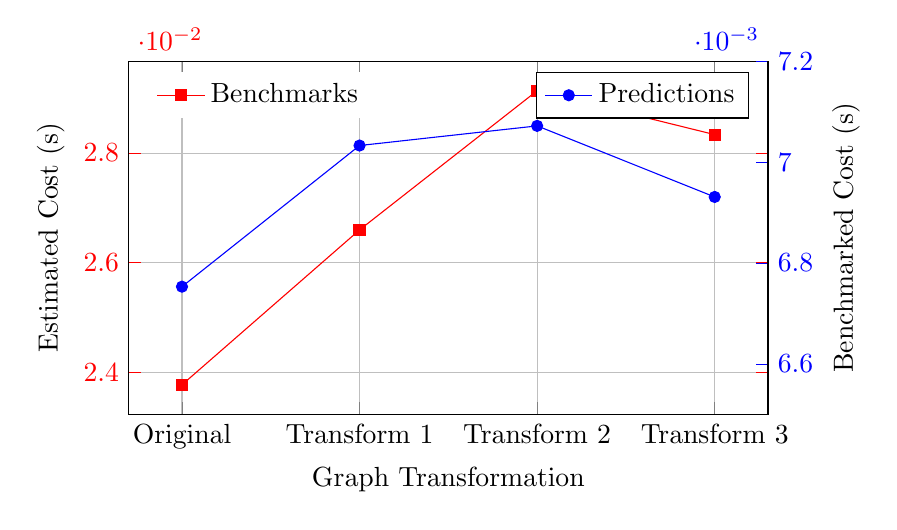
\begin{tikzpicture}
        \begin{axis}[
            xlabel={Graph Transformation}, % X-axis label
            ylabel={Estimated Cost (s)}, % Left Y-axis label
            xtick={1,2,3,4}, % X-ticks for 4 transformations
            xticklabels={Original, Transform 1, Transform 2, Transform 3}, % Custom labels
            legend pos=north west, % Legend position
            grid=both, % Adds a grid
            width=0.8\textwidth, % Adjust plot width
            height=0.5\textwidth, % Adjust plot height
            yticklabel style={color=red}, % Make left Y-axis labels red
            ytick style={color=red}, % Make left Y-ticks red
            legend style={draw=none}, % Remove legend border
        ]
            % Plot the "Actual Cost (s) (Benchmarked)" values
            \addplot[color=red, mark=square*] coordinates {
                (1, 0.0237696305716163)
                (2, 0.026597643813779295)
                (3, 0.029137951823501828)
                (4, 0.028336809511033203)
            };
            \addlegendentry{Benchmarks} % Legend entry for red line
        \end{axis}

        % Add secondary Y-axis
        \begin{axis}[
            axis y line*=right, % Position secondary Y-axis on the right
            axis x line=none, % Hide X-axis for the secondary axis
            ylabel={Benchmarked Cost (s)}, % Right Y-axis label
            ymin=0.0065, ymax=0.0072, % Adjust range for the blue line
            ytick={0.0066, 0.0068, 0.0070, 0.0072}, % Custom ticks for the blue line
            yticklabel style={color=blue}, % Make right Y-axis labels blue
            ytick style={color=blue}, % Make right Y-ticks blue
            width=0.8\textwidth, % Match primary axis width
            height=0.5\textwidth, % Match primary axis height
            legend pos=north east, % Position the secondary legend
        ]
            % Plot the "Estimated Cost (s)" values
            \addplot[color=blue, mark=*] coordinates {
                (1, 0.006753)
                (2, 0.007033)
                (3, 0.007072)
                (4, 0.006931)
            };
            \addlegendentry{Predictions} % Legend entry for blue line
        \end{axis}
    \end{tikzpicture}
    \caption{Comparison of estimated and actual costs with separate scales.}
    \label{resultsPlot}
\end{figure}
As a second example, consider the following equations which show how to optimize the computation involved in a Simple Recurrent Unit as detailed in \cite{jia2019}:
\begin{align*}
&\mathbf{x} \otimes \mathbf{y} + (\mathbf{1} - \mathbf{x}) \otimes \mathbf{z} && \text{(4 operators)} \\
\Rightarrow \, &\mathbf{x} \otimes \mathbf{y} + \mathbf{1} \otimes \mathbf{z} - \mathbf{x} \otimes \mathbf{z} && \text{(5 operators)} \\
\Rightarrow \, &\mathbf{x} \otimes \mathbf{y} - \mathbf{x} \otimes \mathbf{z} + \mathbf{z} && \text{(4 operators)} \\
\Rightarrow \, &\mathbf{x} \otimes (\mathbf{y} - \mathbf{z}) + \mathbf{z} && \text{(3 operators)}
\end{align*}
We begin with a computation that involves 4 operations. Then, the first graph transform increases the number of operations from 4 to 5. This is a degrading transform as the number of operations have increased and we observe a decrease in performance as a result, as shown in Table \ref{resultsTab1}.  However, doing so allows us to discover the form that involves only 3 operations. This would never have been discovered without the initial degrading transform. Thus, this is an application of relaxed graph substitutions at play. We can observe that the final graph has a lower inference time than the initial, showing that the transforms have indeed performed a valid optimization. This has been visualized in Figure \ref{resultsPlot1}.\\
As the main objective was to show that given our backtracking search algorithm (see Algorithm \ref{alg:backtracking}), our cost model is capable of guiding the search to a valid optimization path, we did not focus on implementing the transforms themselves for this example. Each of the 4 forms of the equation have been modeled manually in ONNX and then benchmarked using our cost model. We can see in Figure \ref{resultsPlot} that our cost model accurately portrays the increases and decreases in real inference time, lending accurate ordinality to our measures and helping guide our search to the most optimal model.\\
\begin{table}
        \centering
            \begin{tabular}{|c|c|c|}
                \hline
                Graph & Benchmarked Cost (s) & Estimated Cost (s)\\
                \hline
                Original Model & 0.000706 & 0.00036923 \\
                After Transform 1 & 0.000780 & 0.00054212 \\
                After Transform 2 & 0.000550 & 0.00050784 \\
                After Transform 3 & 0.000446 & 0.00031553 \\
                \hline
            \end{tabular}
            \caption{Running our cost model on the Recurrent Neural Network example. All benchmarking was done using an NVIDIA GeForce RTX 3050 GPU}
            \label{resultsTab1}
\end{table}
        %\vspace{-5mm}
        % Line chart below the table with dual Y-axes
%\vspace{-10mm}
\begin{figure}
    \centering
    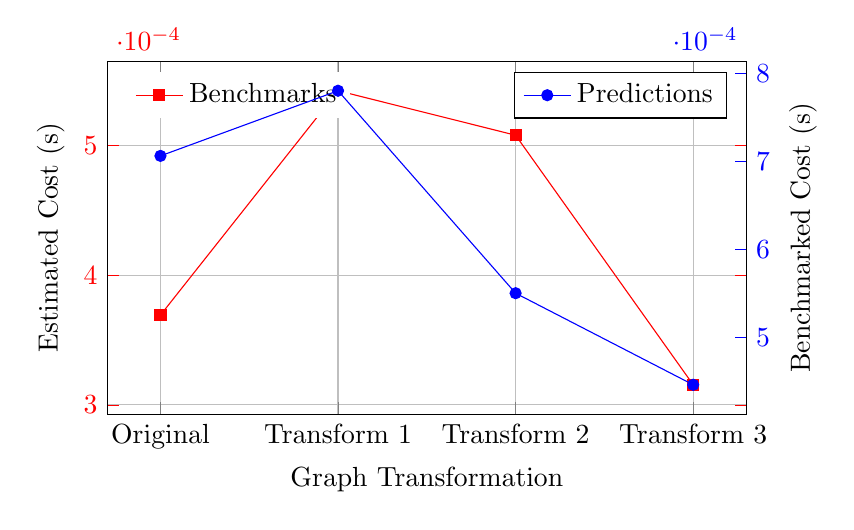
\begin{tikzpicture}
        \begin{axis}[
            xlabel={Graph Transformation}, % X-axis label
            ylabel={Estimated Cost (s)}, % Left Y-axis label
            xtick={1,2,3,4}, % X-ticks for 4 transformations
            xticklabels={Original, Transform 1, Transform 2, Transform 3}, % Custom labels
            legend pos=north west, % Legend position
            grid=both, % Adds a grid
            width=0.8\textwidth, % Adjust plot width
            height=0.5\textwidth, % Adjust plot height
            yticklabel style={color=red}, % Make left Y-axis labels red
            ytick style={color=red}, % Make left Y-ticks red
            legend style={draw=none}, % Remove legend border
        ]
            % Plot the "Actual Cost (s) (Benchmarked)" values
            \addplot[color=red, mark=square*] coordinates {
                (1, 0.0003692278291565046)
                (2, 0.000542119642172257)
                (3, 0.0005078350479065046)
                (4, 0.00031552823540650464)
            };
            \addlegendentry{Benchmarks} % Legend entry for red line
        \end{axis}

        % Add secondary Y-axis
        \begin{axis}[
            axis y line*=right, % Position secondary Y-axis on the right
            axis x line=none, % Hide X-axis for the secondary axis
            ylabel={Benchmarked Cost (s)}, % Right Y-axis label
            %ymin=0.0065, ymax=0.0072, % Adjust range for the blue line
            %ytick={0.0066, 0.0068, 0.0070, 0.0072}, % Custom ticks for the blue line
            yticklabel style={color=blue}, % Make right Y-axis labels blue
            ytick style={color=blue}, % Make right Y-ticks blue
            width=0.8\textwidth, % Match primary axis width
            height=0.5\textwidth, % Match primary axis height
            legend pos=north east, % Position the secondary legend
        ]
            % Plot the "Estimated Cost (s)" values
            \addplot[color=blue, mark=*] coordinates {
                (1, 0.000706)
                (2, 0.000780)
                (3, 0.000550)
                (4, 0.000446)
            };
            \addlegendentry{Predictions} % Legend entry for blue line
        \end{axis}
    \end{tikzpicture}
    \caption{Comparison of estimated and actual costs with separate scales.}
    \label{resultsPlot1}
\end{figure}

\chapter{Conclusion and Future Work}
\section{Conclusion}
In this report, we explained the notion of non-greedy optimizations, motivated their need, and gave an exposition on our attempt at implementing the same, with our work being based on \cite{jia2019}. We saw, using an example, how by allowing intermediate results that are less optimal we can find paths that ultimately lead to graphs better than what we would have obtained using a greedy approach. 

Because individual heuristics for such special cases would lead to a convoluted software, a backtracking algorithm is used to exhaustively search the entire space of graphs enabled by a predetermined set of transformations. At a given iteration, the backtracking algorithm estimates the performance of an intermediate result using a \textit{cost model}, and uses a parameter $\alpha$ to set how relaxed of a substitution we can tolerate, based on factors such as external time-bounds or performance bounds. 

The most crucial part of this work is the cost model. We divided the cost model into three facets:
\begin{enumerate}
    \item Estimate the cost of an individual operator: we do this by (i) finding its lowest possible runtime, $t_{opt}$, by dividing its FLOPS with peak CPU flops, and (ii) dividing this value with the platform percentage of performance(PPP).
    \item We estimate the cost of intermediate writes to and reads from memory, by simply dividing number of bytes with bandwidth, and where bandwidth is estimated using the mbw linux utility.
    \item We then consolidate the layer and memory costs through a heuristic that models model parallelism.
\end{enumerate}

Finally, we compare the estimations made by our cost model to the actual benchmarked values, and see that it is fairly accurate at determining relative costs, which is sufficient for our purposes.

%\begin{enumerate}
 %   \item prepare queue of intermediate results, and set initial graph as the $\mathcal{G}_{optimal}$    %%\item Do until queue of intermediate results empties:
  %  \begin{enumerate}
   %     \item dequeue an intermediate result, apply all transformations on it, and for every transformation that generates a \textit{tolerable} result, add the intermediate result to the queue.
        %\item for every transformation that generates a graph more optimal than $\mathcal{G}_{optimal}$, %set $\mathcal{G}_{optimal}$ to that graph.
 %   \end{enumerate}
%\end{enumerate}
Finally, we present the results comparing the benchmarks obtained via our cost model with actual inference time on real-world hardware.

\section{Future Work}
This work holds a lot of potential yet to be manifested, and we briefly explain the future directions as follows.
As discussed in the results section, we could not test our cost model on graph 5 in the chain because ONNX doesn't support a fused Conv+Relu node. We wish to hence either (i) facilitate this node within ONNX Runntime, or (ii) Port our cost model to Tensorflow RT which \textit{does} implement such a node. We also wish to discover and add more potential downgrading transformations to improve the variety of sequences searched. Our memory model can also be improved, potentially by modeling the memory hierarchy imposed by caches and understanding the ONNX Runtime implementation better for a better FLOPS estimate. Finally, our cost model, while promising, has scope for improvement: We do not have a way of modeling optimizations that ONNX may do, which is to say, when using it one must disable optimizations manually, lest they get unreliable results. Furthermore, the algorithm that models parallelism currently assumes that there's always a new thread available --- i.e. that there are infinite threads. This works alright when optimizing small graphs, but will be problematic when optimizing large graphs with many branches.

Our current efforts at implementation can be seen on our public GitHub repository \footnote{https://github.com/thehthakur/Take\_It\_Easy/tree/main}.
    
\appendix

\chapter{Diving Into The ResNet Example}
\section{Diving Into the Transformations}
		% tensorflow didn't have transforms we could work off of, so went with the paper's example
		% deep dive in the transforms
\begin{figure}[ht!]
    \begin{center}
	      \includegraphics[scale=0.3]{reportImages/resnetExample.png}   
    \end{center}	
    \caption{An example introduced in section 3 and taken from \cite{jia2019}}
	\label{resnet_jia}
\end{figure}
 
 Initially, we wanted to look for graph transformations that were already available in any of the deep learning frameworks, such as PyTorch, TensorFlow, etc. But after going deep into the implementations of the transformations provided by the TensorFlow XLA, we noticed that every transformation provided by the deep learning frameworks always improves performance and never degrades it, which dismisses the prospect of relaxed substitutions. Hence, we decided to implement the transformations provided in the \cite{jia2019}, as shown in figure \ref{resnet_jia}.
		% tensorflow didn't have transforms we could work off of, so went with the paper's example
		% deep dive in the transforms

\subsection{Kernel Expansion}

% enlarge conv kernel figure
\begin{figure}[ht]
\centering
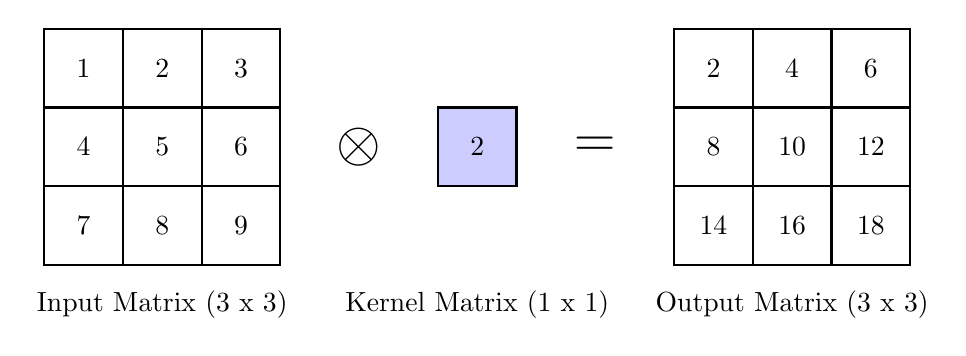
\begin{tikzpicture}
    % Define the block size
    \def\blocksize{1}

    \foreach \i in {0, 1, 2} {
        \foreach \j in {0, 1, 2} {
            \pgfmathtruncatemacro\result{(2-\j)*3+\i+1}
            \draw[thick] (\i*\blocksize, \j*\blocksize) rectangle +(\blocksize, \blocksize);
            \node at (\i*\blocksize + 0.5*\blocksize, \j*\blocksize + 0.5*\blocksize) {\result};
        }
    }

    \node at (4.0, 1.5) {\huge $\otimes$};

    \draw[thick, fill=blue!20] (5.0, 1.0) rectangle +(\blocksize, \blocksize);
    \node at (5.0 + 0.5*\blocksize, 1.0 + 0.5*\blocksize) {2};

    \node at (7.0, 1.5) {\huge =};

    \foreach \i in {0, 1, 2} {
        \foreach \j in {0, 1, 2} {
            \pgfmathtruncatemacro\result{((2-\j)*3+\i+1)*2}
            \draw[thick] (8.0 + \i*\blocksize, \j*\blocksize) rectangle +(\blocksize, \blocksize);
            \node at (8.0 + \i*\blocksize + 0.5*\blocksize, \j*\blocksize + 0.5*\blocksize) {\result};
        }
    }

    % Labels
    \node at (1.5, -0.5) {Input Matrix (3 x 3)};
    \node at (5.5, -0.5) {Kernel Matrix (1 x 1)};
    \node at (9.5, -0.5) {Output Matrix (3 x 3)};

\end{tikzpicture}

\label{kernelExpansion0}
\caption{Convolution Operation with a 1x1 kernel matrix, a padding of zero, and stride 1}
\end{figure}

\begin{figure}[ht]
\centering
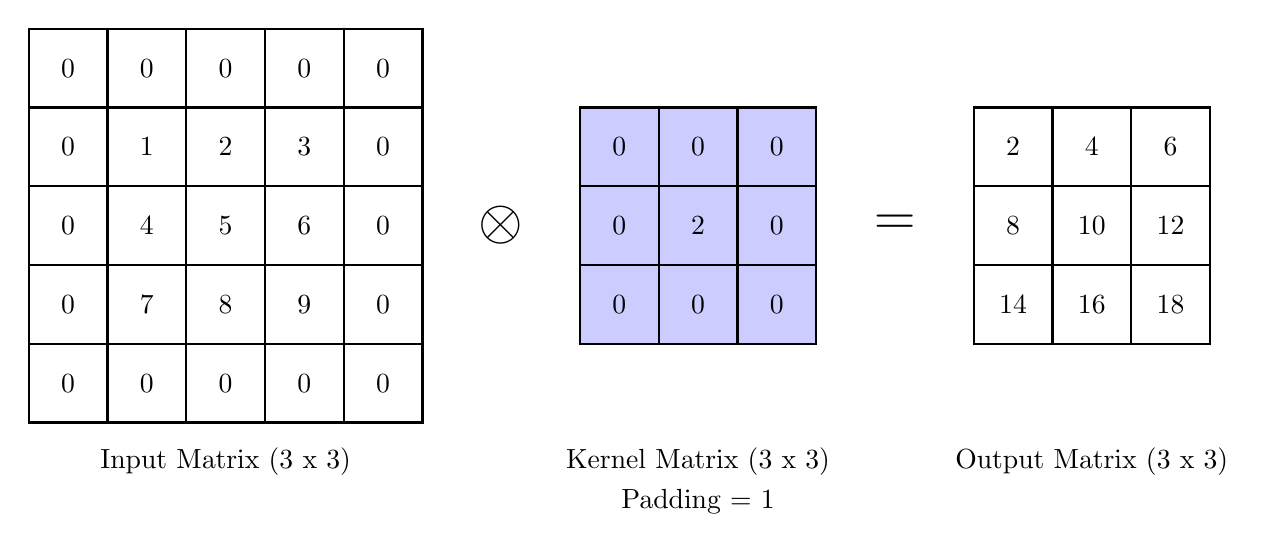
\begin{tikzpicture}
    % Define the block size
    \def\blocksize{1}

    \foreach \i in {0, 1, 2, 3, 4} {
        \foreach \j in {0, 1, 2, 3, 4} {
            \pgfmathtruncatemacro\result{(3-\j)*3+\i}
            \pgfmathtruncatemacro\finalresult{ifthenelse(\i==0 || \j==0 || \i==4 || \j==4, 0, \result)} % Apply conditions
            \draw[thick] (\i*\blocksize, \j*\blocksize) rectangle +(\blocksize, \blocksize);
            \node at (\i*\blocksize + 0.5*\blocksize, \j*\blocksize + 0.5*\blocksize) {\finalresult};
        }
    }

    \node at (6.0, 2.5) {\huge $\otimes$};

    \foreach \i in {0, 1, 2} {
        \foreach \j in {0, 1, 2} {
            \pgfmathtruncatemacro\result{0}
            \pgfmathtruncatemacro\finalresult{ifthenelse(\i==1 && \j==1, 2, \result)} % Apply conditions
            \draw[thick, fill=blue!20] (7 + \i*\blocksize, 1 + \j*\blocksize) rectangle +(\blocksize, \blocksize);
            \node at (7 + \i*\blocksize + 0.5*\blocksize, 1 + \j*\blocksize + 0.5*\blocksize) {\finalresult};
        }
    }

    \node at (11.0, 2.5) {\huge =};

    \foreach \i in {0, 1, 2} {
        \foreach \j in {0, 1, 2} {
            \pgfmathtruncatemacro\result{((2-\j)*3+\i+1)*2}
            \draw[thick] (12.0 + \i*\blocksize, 1.0 + \j*\blocksize) rectangle +(\blocksize, \blocksize);
            \node at (12.0 + \i*\blocksize + 0.5*\blocksize, 1.0 + \j*\blocksize + 0.5*\blocksize) {\result};
        }
    }

    % Labels
    \node at (2.5, -0.5) {Input Matrix (3 x 3)};
    \node at (8.5, -0.5) {Kernel Matrix (3 x 3)};
    \node at (8.5, -1.0) {Padding = 1};
    \node at (13.5, -0.5) {Output Matrix (3 x 3)};

\end{tikzpicture}

\label{kernelExpansion1}
\caption{A convolution operation after padding both, the kernel and the image.}
\end{figure}

               The substitution \verb|enlarge_conv_kernel| increases the kernel size from 1x1 to a larger 3x3 size. This change enables further transformations that can lead to improved performance. However, as previously mentioned, simply increasing the kernel size does not guarantee correctness. \\

              Let us assume the initial kernel size is $f$, and the final kernel size is $f+k$, where we are increasing the kernel size by $k$. The initial padding is $p$, and the final padding is $p'$. The input size is $n$.

               \begin{equation}
                    \frac{n+2p-f}{s} + 1 = \frac{n+2p^\prime-(f+k)}{s} + 1
                \label{eq:enlarge1}
                \end{equation}

                \begin{equation}
                    2p-f= 2p^\prime-(f+k)
                \label{eq:enlarge2}
                \end{equation}

                \begin{equation}
                    \boxed{p^\prime = p + \frac{k}{2}}
                \label{eq:enlarge2}
                \end{equation}

                Hence, enlarging the kernel will also require adding padding to the input in the convolution operation to maintain the same output dimensions.

            \subsection{Convolution Fusions}
            Convolution Fusions combine multiple convolution oeprations into a single, more efficient oepration. This approach aims to reduce the number of operations and memory access overhead by merging sequential convolutional layers.

    \begin{figure}[ht]
    \centering
    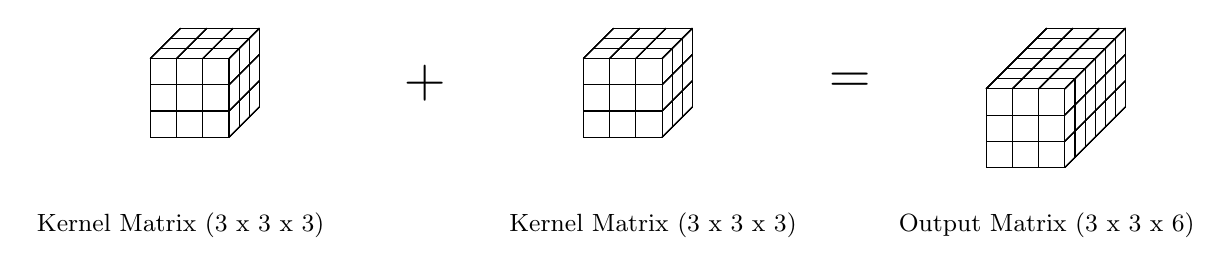
\begin{tikzpicture}
        % First Cube
        \foreach \x in {0, 1, 2, 3} {
            \foreach \y in {0, 1, 2, 3} {
                \draw (2.5 + 0, \y/3, 3/3) -- (2.5 + 3/3, \y/3, 3/3); % Horizontal lines
                \draw (2.5 + \y/3, 0, 3/3) -- (2.5 + \y/3, 3/3, 3/3); % Vertical lines on YZ plane
                \draw (2.5 + 3/3, \y/3, 3/3) -- (2.5 + 3/3, \y/3, 0); % Vertical lines on XZ plane
                \draw (2.5 + \y/3, 3/3, 3/3) -- (2.5 + \y/3, 3/3, 0); % Horizontal lines on XY plane
                \draw (2.5 + 3/3, 0, \y/3) -- (2.5 + 3/3, 3/3, \y/3); % Vertical lines on XZ plane
                \draw (2.5 + 0, 3/3, \y/3) -- (2.5 + 3/3, 3/3, \y/3); % Horizontal lines on XY plane
            }
        }

        \node at (5.6, 0.3) {\huge +};

        % Second Cube
        \foreach \x in {0, 1, 2, 3} {
            \foreach \y in {0, 1, 2, 3} {
                \draw (8.0, \y/3, 3/3) -- (8.0 + 3/3, \y/3, 3/3); % Horizontal lines
                \draw (8.0 + \y/3, 0, 3/3) -- (8.0 + \y/3, 3/3, 3/3); % Vertical lines on YZ plane
                \draw (8.0 + 3/3, \y/3, 3/3) -- (8.0 + 3/3, \y/3, 0); % Vertical lines on XZ plane
                \draw (8.0 + \y/3, 3/3, 3/3) -- (8.0 + \y/3, 3/3, 0); % Horizontal lines on XY plane
                \draw (8.0 + 3/3, 0, \y/3) -- (8.0 + 3/3, 3/3, \y/3); % Vertical lines on XZ plane
                \draw (8.0, 3/3, \y/3) -- (8.0 + 3/3, 3/3, \y/3); % Horizontal lines on XY plane
            }
        }

        \node at (11, 0.3) {\huge =};

        % Cuboid (with correction)
        \foreach \x in {0, 1, 2, 3} {
            \foreach \y in {0, 1, 2, 3} {
                % Draw the front face
                \draw (13.5, \y/3, 2) -- (13.5 + 1, \y/3, 2); % Top horizontal on front face
                \draw (13.5 + \y/3, 0, 2) -- (13.5 + \y/3, 1, 2); % Side vertical on front face
                \draw (13.5 + 1, \y/3, 2) -- (13.5 + 1, \y/3, 0); % Right vertical on front face
                \draw (13.5 + \y/3, 1, 2) -- (13.5 + \y/3, 1, 0); % Bottom horizontal on front face

            }
        }

        % Add height edges for the depth of the cuboid
                \draw (13.5 + 1, 0, 2/6) -- (13.5 + 1, 0+1, 2/6); % Right front vertical edge
                \draw (13.5 + 1, 0, 4/6) -- (13.5 + 1, 0+1, 4/6); % Right front vertical edge
                \draw (13.5 + 1, 0, 6/6) -- (13.5 + 1, 0+1, 6/6); % Right front vertical edge
                \draw (13.5 + 1, 0, 8/6) -- (13.5 + 1, 0+1, 8/6); % Right front vertical edge
                \draw (13.5 + 1, 0, 10/6) -- (13.5 + 1, 0+1, 10/6); % Right front vertical edge
                \draw (13.5 + 1, 0, 0) -- (13.5 + 1, 0+1, 0); % Right front vertical edge

                \draw (13.5, 1, 1) -- (13.5+1, 1, 1); % Top horizontal on front face
                \draw (13.5, 1, 2/6) -- (13.5+1, 1, 2/6); % Top horizontal on front face
                \draw (13.5, 1, 4/6) -- (13.5+1, 1, 4/6); % Top horizontal on front face
                \draw (13.5, 1, 8/6) -- (13.5+1, 1, 8/6); % Top horizontal on front face
                \draw (13.5, 1, 10/6) -- (13.5+1, 1, 10/6); % Top horizontal on front face
                \draw (13.5, 1, 0) -- (13.5+1, 1, 0); % Top horizontal on front face

    \node at (2.5, -1.5) {\small Kernel Matrix (3 x 3 x 3)};
    \node at (8.5, -1.5) {\small Kernel Matrix (3 x 3 x 3)};
    \node at (13.5, -1.5) {\small Output Matrix (3 x 3 x 6)};

    \end{tikzpicture}

	\label{convFusion0}
	\caption{Fusing two kernel matrices}
\end{figure}

            The fusing of convolution layers can only be done if the following conditions are satisfied:

            \begin{tcolorbox}[colback=gray!5!white, colframe=gray!75!black, title=Constraints on the Source Graph]
            \begin{itemize}[left=0pt]
                \item \verb|conv1.kernel == conv2.kernel|
                \item \verb|conv1.stride == conv2.stride|
                \item \verb|conv1.padding == conv2.padding|
            \end{itemize}
        \end{tcolorbox}
        
        \begin{tcolorbox}[colback=gray!5!white, colframe=gray!75!black, title=Construct the Target Graph]
            \begin{itemize}[left=0pt]
                \item \verb|conv3.outChannels = conv1.outChannels + conv2.outChannels|
                \item \verb|conv3.weights = concat(conv1.weights, conv2.weights)|
                \item \verb|split.sizes = [conv1.outChannels, conv2.outChannels]|
            \end{itemize}
        \end{tcolorbox}

\subsection{Fusing Conv and Add Nodes}
	  One of the more non-obvious and harder to unpack transformations proved to be the fusion of a Convolutional node and an Add node. The process is best understood by first revisiting concepts of Convolution networks.
	  \begin{figure}[b!]
		\begin{center}
			\includegraphics[scale=0.3]{reportImages/CNN_revision_bishop.png}
		\end{center}	
		\caption{An illustration from \cite{bishop2023deep} that shows a  multi-dimensional convolutional filter layer extended to include multiple independent filter channels.}
		\label{cnn_revision}
	\end{figure}
	  \begin{itemize}
		\item An image with $J \times K$ pixels and C channels will be described by a tensor of dimensionality $J \times K \times C$. We introduce a filter described by a tensor of dimensionality $M \times M \times C$ comprising a separate $M \times M$ filter for each of the C channels.
		\item Secondly, we introduce multiple such filters, each detecting a seperate abstract feature in the input image. The number of these specific filters are referred to as the channels of the kernel and are denoted by the third number in the notation $3 \times 3 \times 512$ for a convolutional layer.
		\item For each filter, after performing the convolution operation across all channels of the input image, the resulting C channels are summed to produce the final feature map representing the abstract feature the filter is designed to detect.
	\end{itemize}

	Now with the basis of the convolutional approach laid down, we can explore the optimization. The input is a $3 \times 3 \times 512$ image which was formed after fusing two $3 \times 3 \times 256$ convolutional operations together. The first 256 channels out of the 512 denote the input that came from Conv1 and the rest 256 denote the channels that came from Conv2. As Figure \ref{resnet} shows, the expected behaviour is for the Conv1 channels to undergo one more convolution, say Conv4, and then simply get added to the Conv2 output.

	The optimization here is to cleverly modify the kernel matrix of a new Conv operation, call it Conv3, that includes within it the Convolution operation on Conv1 channels and subsequent addition. The approach is as follows:
	  \begin{itemize}
		\item In Conv3, there are 256 different filters. Each of these filters is responsible for extracting some abstract feature.
		\item Each of these filters has 512 channels, 256 devoted to processing the channels consolidated from Conv1 and the remaining 256 for processing the add.
		\item Note that each filter within the Conv4 layer has 256 channels within it to handle the 256 input channels from Conv1.
		\item The fusion is accomplished in two steps. The first is to have the first 256 channels of Conv3 be initialized with the weights of the corresponding channel in the $3 \times 3 \times 256$ Conv4.
		\item Now, we know that, per abstract feature, after carrying convolution over all channels, the final feature map is a result of summing up over all the channels. In our current arrangement the first 256 channels, when summed up, will give the output feature map corresponding to performing Conv4 for that abstract feature. The remaining part is to add to this sum precisely the channel that corresponds to Conv2, that, when added, will simulate doing a sum post convolution.
		\item The trick here is to use the \textbf{identity kernel}, which simply outputs the input as is without modification. It is also called a do-nothing kernel.
		\[ I = 
	\begin{bmatrix}
	0 & 0 & 0 \\
	0 & 1 & 0 \\
	0 & 0 & 0
	\end{bmatrix}
	\]
		\item Let us make a few constructs:
		\begin{itemize}
			\item Let 0 represent a 3x3 kernel filled with all zeros.
			\item Let each row of the matrix represent the kernel corresponding to one of the 256 abstract features in Conv3.
			\item Let $f_{i,j}$ denote a $k \times k$ filter for abstract feature $i$ and channel $j$.
		\end{itemize} . 
		\[
			\begin{bmatrix}
					f_{1,1} & f_{1,2} & f_{1,3} & \cdots & f_{1,256} & I & 0 & 0 & \cdots & 0\\
					f_{2,1} & f_{2,2} & f_{2,3} & \cdots & f_{2,256} & 0 & I & 0 & \cdots & 0\\
					\vdots & \vdots & \vdots & \vdots & \vdots & \vdots & \vdots & \vdots & \cdots & \vdots \\
					f_{256,1} & f_{256,2} & f_{256,3} & \cdots & f_{256,256} & 0 & 0 & 0 & \cdots & I
			\end{bmatrix}
	\]
	\item The above kernel matrix can be seen as the original Conv4 weight matrix concatenated with an "Identity" matrix. This identity matrix is actually a matrix of matrices where the diagonal elements are identity kernels.
	\end{itemize}
	By configuring the last 256 channels to either the identity matrix  $I$ or zero, as shown in the matrix above, we can selectively sum the layers that would have been added in the original computational graph.





%\begin{enumerate}

	%\item The first step would be to finalize a set of graph transformations we will be working with (i.e. the set $T$ in the earlier algorithm). We initially construted the initial computation graph shown in figure \ref{resnet} using the ONNX Python API \cite{onnxpython}, and explored the graph transformations made available by the ONNX Optimizer \cite{onnxoptimizer} through a simple backtracking algorithm. That being said, since ONNX provides \textit{optimizations} and not \textit{transformations}, each available transform is bound to improve performance for most if not all input graphs. This renders the purpose of our algorithm moot. This is why, we now plan to explore the transformations made available through the TensorFlow \cite{tf2016} API which also provides a tool to write custom transforms.
	%\item Once a set of Tensorflow transforms are shortlisted, we can move on to analyze the feasibility of, and then potentially implement, the two latter transforms mentioned in figure \ref{resnet}, which currently don't have implementations in TensorFlow. 
	%\item We then create a test suite consisting of small computation graphs that demonstrate the abilities of our algorithm.
	%\item Once the aforementioned stages are successful, we will then benchmark our backtracking implementation against the aforementioned test suite, and analyze the results.
	%\item Based on the results obtained, we then aim to tweak the cost model that approximates the cost function for an input graph so as to consider other parameters such as FLOPS or memory consumed.
	%\item The above steps will hopefully yield a model that is successful with regard to small input computation graphs. In order to scale this system to work for existing models, which have massive computation graphs that are bound to blow up the search space exponentially, we plan to create a \textit{graph splitting} algorithm that divides the computation graph into smaller sub-graphs. Each sub-graph can then be optimized through the earlier algorithm. In \cite{jia2019}, the metric used to find partitioning-boundaries is a parameter called $Cap(N)$, which, for a given node $N$, tells us the number of graph transformations thwarted if the graph were split through this node. Since we want the least number of thwarted transforms, the paper then uses the max-flow algorithm \cite{cormen2009introduction} to find partitioning boundaries.
	%\item The paper also mentioned that this min-cut algorithm is not necessarily optimal for all models. Hence, there is scope of improvement with regard to defining better graph-splitting heuristics. We see this as possible future work.

%\end{enumerate}

%\addcontentsline{toc}{chapter}{References}
\bibliographystyle{plain}
\bibliography{refs}

%\begin{center}
%\begin{tabular}{@{}p{.5in}p{4in}@{}}
%& \hfill \\
%& \hfill \\
%& \hrulefill \\
%& Shri. R. P. Gohil \\
%& Associate Professor, DoCSE, SVNIT\\
%\end{tabular}
%\end{center}

\chapter*{Acknowledgements}
\addcontentsline{toc}{chapter}{Acknowledgements}

Any palpable progress with this work wouldn't have been possible without Prof. R. P. Gohil's guidance on a very fundamental level: we needed to base our goals on a concrete feasibility analysis rather than quixotic assumptions of glory. We really did face quite a few contingencies even after narrowing our focus down to something realistic, but, thanks to his prudent reminders, we now have some measurable progress.

\end{document}
